\documentclass[
 preprint,
 preprintnumbers,
 amsmath,amssymb,
 aps,
 pre,
 longbibliography,
 superscriptaddress,
 10pt, twocolumn
]{revtex4-1}



\usepackage{graphicx}% Include figure files
\graphicspath{{./figures/}} % path to figures
\usepackage{dcolumn}% Align table columns on decimal point
\usepackage{bm}% bold math
\usepackage{hyperref}% add hypertext capabilities
\usepackage{physics} % package for physics symbols
\usepackage{color}
\begin{document}
% define commands
\newcommand{\eqnname}{Eqn.}
\newcommand{\secname}{Sec.}


\title{Rectification of energy and motion in active gyroscopic networks}


\author{Zhenghan Liao}
\affiliation{Department of Chemistry, University of Chicago, Chicago, IL, 60637, USA}
\author{William Irvine}
\affiliation{James Franck Institute, Enrico Fermi Institute and Department of Physics, University of Chicago, Chicago, IL, 60637, USA}
\author{Suriyanarayanan Vaikuntanathan}
\affiliation{James Franck Institute and Department of Chemistry, University of Chicago, Chicago, IL, 60637, USA}


\begin{abstract}
[Will be revised in the end] We study a model that combines gyroscopic networks and active matter. From numerical calculations, theory, and simulations, we show that autonomous heat flows are generated at the nonequilibrium steady state. Distinct from conventional heat flows that are driven by temperature difference at the boundaries, this heat flow is an emergent collective behavior.
We then focus on understanding three issues: the mechanism of this nonzero heat flow, the connection between the flow in active system and that in the well-studied isolated system, and the relationship between the network geometry and the flow pattern.
Understanding the last issue in turn enables us to control the flow pattern by the design of the network geometry.
\end{abstract}

\maketitle

\section{Introduction} \label{sec:intro}
% ==============================================================================
% Suri's intro
% One of the longstanding problems in non-equilibrium statistical mechanics concerns uncovering principles for the rectification of energy and motion in many body microscopic systems~\cite{seifert2012stochastic,coskun2012great}. The Feynman Ratchet and pawl model, and its associated generalizations, have elucidated how a combination of spatial asymmetry and non-equilibrium forcing can lead to rectification of current and work generation in simple low dimensional model systems~\cite{jarzynski1999feynman}. Brownian ratchet models have also provided a framework to understand how molecular motors and biophysical polymers like actin transmit and exert forces~\cite{mogilner1996cell}. New theoretical results, such as the no pumping theorems have provided a minimal set of constraints for changing the kinetic rates in a ratchet model to ensure rectification~\cite{Chernyak2008,Rahav2008,Sinitsyn2007}. Despite these advances, we still have very few design principles to engineer rectification in many body systems~\cite{seifert2012stochastic}. This is a current and relevant problem of interest, especially given the recent progress made in the in study of so called active matter systems where energy injection at the microscopic level results in larger scale reorganization ~\cite{marchetti2013hydrodynamics,souslov2017topological,Shankar2017}.In this paper, we attempt to address a limited version of the problem and show energy and motion can be rectified in a class of model systems composed of chiral meta-materials interacting with an active bath.
%
% Designs of mechanical metamaterials have achieved unconventional mechanical properties or functions in a wide range of systems \cite{Bertoldi2017FlexibleMechanical}. Examples include negative Poisson ratios in auxetic metamaterials \cite{Lakes2017NegativePoissonSRatio,Ren2018AuxeticMetamaterials}, topological zero modes in isostatic lattices \cite{Kane2013TopologicalBoundary,Lubensky2015PhononsElasticity,Paulose2015SelectiveBuckling}, unidirectional edge modes in topological gyroscopic metamaterials \cite{Nash2015TopologicalMechanics,Wang2015TopologicalPhononic,Mitchell2018AmorphousTopological}, and the allosteric effect in mechanical networks \cite{Rocks2017DesigningAllosteryinspired,Yan2017ArchitectureCoevolution,Flechsig2017DesignElastic}. In particular, studies of gyroscopic chiral metamaterials have shown how peculiar topological edge modes, where the energy circulates along the network boundary unidirectionally, can be supported in classical systems\cite{Nash2015TopologicalMechanics}. These topological chiral edge modes can be explained in terms of a violation of time reversal symmetry in the microscopic equations of motion of the interacting gyroscopes~\cite{Nash2015TopologicalMechanics,Mitchell2018AmorphousTopological}. Importantly, the violation of time reversal symmetry is controlled by an interplay between the spin of the gyroscopes and the geometry of the lattice.
%
% %In contrast to the increasing studies on mechanical properties, one less explored topic is the effect of thermal fluctuations{\bf rewrite sentence, awkward construction}. This effect is usually irrelevant, because the energy scale of the metamaterials is much larger than that of thermal fluctuations. However, fluctuations are inevitable if the system is made in micro-scale \cite{Blees2015GrapheneKirigami}.
% % Indeed, some recent works have found an interesting interplay between thermal \cite{Rocklin2018FoldingMechanisms,Pedro2018TopologicalProtection} or nonequilibium \cite{Woodhouse2018AutonomousActuation} fluctuations and the zero mode, which show promises in studying the effect of fluctuations.
%
% In this paper we show how notions of time reversal symmetry violation in chiral topological metamaterials can be combined with violations of the fluctuation dissipation relation by \textit{active} particles to rectify energy and mass flows. The active bath we use is the active Ornstein-Uhlenbeck particle (AOUP) model \cite{Fodor2016HowFar}, which consists of a constant friction and an Ornstein-Uhlenbeck (OU) noise. The AOUP model has experienced a growing interest in recent years, because of its theoretical simplicity and its ability to capture many nonequilibrium and active matter phenomena.
% For instance, it has been experimentally found that, colloids in a bacteria bath can be well-modeled by the AOUP model \cite{Wu2000ParticleDiffusion}; this finding helped realized previously proposed thermal ratchet models \cite{Magnasco1993ForcedThermal} in experiments with bacterial baths. \cite{Koumakis2013TargetedDelivery}
%
% Our central result shows how a combination of time reversal symmetry violations due to chirality and interactions in a model system, and time reversal symmetry violations implicit in the fluctuations of the bath that the model system is in contact with, can help support rectification. In particular, we find that our combined system can support a directed flux of energy across the network. Unlike conventional energy flows, our energy flow is not supported by a temperature gradient. Moreover, the \textit{active gyroscopic} network can in fact pump energy through an otherwise isolated elastic object. We also show that the microscopic mechanisms responsible for this energy flow can also potentially allow the \textit{active gyroscopic} network to swim in and exert forces on a viscous fluid. We analytically and numerically demonstrate these results for a wide variety of network geometries thus establishing the generality of our results. In particular, we construct an intuitive diagrammatic approach for computing the energy flux (and consequently the swim speed) that shows how our results can readily applied to tailor flows in arbitrarily complex networks.
%
% Taken together, our results establish a new set of design principles for rectification of energy, motion and forces in chiral many body systems. Our design principles, unlike many existing prescriptions, exploit inherent asymmetries in the geometry and interactions of the material to achieve rectification.
% ==============================================================================

[{\bf New combined introduction: by Suri}] 

Uncovering principles that can enable the rectification of stochastic fluctuations has been a long standing problem in non-equilibrium statistical mechanics. ~\cite{Seifert2012StochasticThermodynamics,Coskun2011GreatExpectations}. The Feynman Ratchet and pawl model, and its associated generalizations, have elucidated how systems that can rectify stochastic fluctuations can act as microscopic engines that perform work and exert forces~\cite{Jarzynski1999FeynmanRatchet}. Indeed such models have provided a framework to understand how biological molecular motors can rectify stochastic fluctuations, and convert the energy derived from the hydrolysis of energy rich molecules into mechanical work~\cite{Mogilner1996CellMotility,Chernyak2008PumpingRestriction,Rahav2008DirectedFlow,Sinitsyn2007UniversalGeometric}. While these advances provide powerful design principles, especially for rectification in single-body systems, we still have very few design principles to engineer rectification in many body systems~\cite{Seifert2012StochasticThermodynamics}, particularly in the absence of any imposed asymmetries.Uncovering such principles can, for instance, identify methods to manipulate the flow of energy across materials without any imposed temperature biases~\cite{Dubi2011ColloquiumHeat,Strohm2005PhenomenologicalEvidence,Li2012ColloquiumPhononics,Kanazawa2013HeatConduction,Morgado2016ThermostatisticsSmall,Martinez2017ColloidalHeat}. They can also potentially facilitate the development of design principles for constructing synthetic molecular motor analogues. In this paper, we establish a new and general set of principles for how such rectification can be achieved in many body interacting systems. In particular, we show how a parity violating meta material~\cite{Nash2015TopologicalMechanics} can spontaneously rectify energy and motion in the absence of any imposed gradients, when it is allowed to interact with a bath of \textit{active} particles that consume energy to power their motion~\cite{Marchetti2013HydrodynamicsSoft,Souslov2017TopologicalSound,Shankar2017TopologicalSound}. 

%we show how phonons generated in a parity violating meta material~\cite{Nash2015TopologicalMechanics}, when allowed to interact with a bath of \textit{active} particles that consume energy to power their motion~\cite{Marchetti2013HydrodynamicsSoft,Souslov2017TopologicalSound,Shankar2017TopologicalSound}, can spontaneously rectify energy and motion in the absence of any externally imposed gradient. 

%Our analytical calculations identify the important ingredients necessary for rectification. In particular, they show how a combination of non-equilibrium activity at the single particle level can exploit inherent asymmetries in the geometry and interactions of the chiral meta material to achieve rectification of energy and motion. %In this manner, our results 

We construct our design principles using a class of model parity violating meta materials. Our choice of parity violating meta material is inspired by a recent work where a meta material composed of interacting gyroscopes was introduced~\cite{Nash2015TopologicalMechanics}. These gyroscopic meta materials were shown to support chiral topological edge modes. The topological chiral edge modes can be explained in terms of a violation of time reversal symmetry in the microscopic equations of motion of the interacting gyroscopes~\cite{Nash2015TopologicalMechanics,Mitchell2018AmorphousTopological}. Importantly, the violation of time reversal symmetry is controlled by an interplay between the spin of the gyroscopes and the geometry of the lattice. In the model systems considered in this paper, such parity violating meta materials are allowed to interact with a bath of \textit{active} particles that violate the fluctuation dissipation relation~\cite{Fodor2016HowFar}. %Isolated variants of the the parity violating meta material we consider were previously studied in Ref~\cite{Nash2015TopologicalMechanics}. where it was shown to support topological edge modes.


Our central result shows how a combination of time reversal symmetry violations due to chirality, interactions between the particles of our model system, and time reversal symmetry violations implicit in the single particle fluctuations of the bath that the model system is in contact with, can help rectify stochastic fluctuations. Indeed, naively coupling the topological chiral meta material to a heat bath does not result in any fluxes or symmetry breaking on account of the Bohr-van Leeuwen theorem that forbids any non-equilibrium currents in thermalized magnetic systems. In contrast, we find that our model system can support a directed flux of energy across the network. Unlike conventional energy flows, our energy flow is not supported by a temperature gradient. Moreover, we show that the \textit{parity violating active} network can in fact pump energy through an otherwise isolated elastic object. Finally, we also show that the microscopic mechanisms responsible for this energy flow can also potentially allow the \textit{parity violating active} network to swim in and exert forces on a viscous fluid. We analytically and numerically demonstrate these results for a wide variety of network geometries thus establishing the generality of our results. In particular, we construct an intuitive diagrammatic approach for computing the energy flux (and consequently the swim speed) that shows how our results can readily applied to tailor flows in arbitrarily complex networks. Taken together, our results establish a new set of design principles for rectification of energy, motion and forces in chiral many body systems. Our design principles, unlike many existing prescriptions, exploit inherent asymmetries in the geometry and interactions of the material to achieve rectification.



%Our results establish a new set of design principles for rectification in many body systems. Our design principles, unlike many existing prescriptions, exploit inherent asymmetries in the geometry and interactions of the material to achieve rectification.


%[{\bf Zhenghan: intro with focus on energy transport between identical terminals}]

%Conventional heat transport is controlled by temperature biases, i.e., heat flows spontaneously from hot to cold.
%Manipulating the heat flow under temperature biases or discovering new energy conduction mechanisms has been a vibrant area of research.
%A classic discovery is the thermoelectric effect, where a heat flux can be induced by electric currents \cite{Dubi2011ColloquiumHeat}.
%Recent advances in manipulating phonons include applying magnetic fields as in phonon Hall effect \cite{Strohm2005PhenomenologicalEvidence,Li2012ColloquiumPhononics}, exploiting nonlinearity as in thermal diodes \cite{Terraneo2002ControllingEnergy,Li2012ColloquiumPhononics}, coupling phonons to photons \cite{Seif2017ThermalManagement,Safavi-Naeini2019ControllingPhonons}, using time-periodic controls \cite{Li2008RatchetingHeat,Ren2010EmergenceControl,Ren2012GeometricHeat}, utilizing topological materials \cite{Rivas2017TopologicalHeat,Ronetti2017PolarizedHeat,Liu2017ModelTopological,Chien2018TopologicalQuantization}, and introducing nontrivial bath statistics \cite{Kanazawa2013HeatConduction,Morgado2016ThermostatisticsSmall,Martinez2017ColloidalHeat}.
%In most examples, energy is transported between terminals that differ in temperature or other aspects.
%In this paper, we ask how energy flows can be generated and controlled where all sites are identical. Such system will contribute a flexible way to manipulate energy flows. One can imagine that, in a network with a large number of sites, energy fluxes can be manipulated without having to adjust the temperature on each site.
%In a different context of thermal radiation, energy flux between identical sites has been realized at a small scale using nonreciprocal magneto-optical nanoparticles \cite{Zhu2016PersistentDirectional,Zhu2018TheoryManybody,Ott2018CircularHeat}.
%We approach the above question by combining chiral phonons from mechanical metamaterials \cite{Nash2015TopologicalMechanics} with nontrivial bath statistics from active matter \cite{Fodor2016HowFar}.
%The resulting model is a network composed of identical chiral active sites, without applied temperature or other biases.
%We show that this model can support energy transport between its sites, and the energy fluxes can be controlled by the geometry of the network. Furthermore, the same control principle applies to networks with arbitrary geometries and topologies.
%The energy transport without obviously imposed biases can be termed as energy rectification. Unlike many rectification examples that can be understood at a few-body level such as Feynman's ratchet and pawl \cite{Feynman2015FeynmanLectures,Reimann2002BrownianMotors,Martinez2017ColloidalHeat}, this rectification belongs to a many-body class \cite{Asban2014NopumpingTheorem,Reichhardt2017RatchetEffects}. We further show that the energy rectification implicates motion rectification when the network is coupled to a low Reynolds number fluid.


%[intro with focus on rectification in many-body systems]

%One of the longstanding problems in non-equilibrium statistical mechanics concerns uncovering principles for the rectification of energy and motion in microscopic systems~\cite{Seifert2012StochasticThermodynamics,Coskun2011GreatExpectations}. The Feynman Ratchet and pawl model, and its associated generalizations, have elucidated how a combination of spatial asymmetry and non-equilibrium forcing can lead to rectification of current and work generation in simple low dimensional model systems~\cite{Jarzynski1999FeynmanRatchet}. Brownian ratchet models have also provided a framework to understand how molecular motors and biophysical polymers like actin transmit and exert forces~\cite{Mogilner1996CellMotility}. New theoretical results, such as the no pumping theorems have provided a minimal set of constraints for changing the kinetic rates in a ratchet model to ensure rectification~\cite{Chernyak2008PumpingRestriction,Rahav2008DirectedFlow,Sinitsyn2007UniversalGeometric}.
%These advances provide powerful design principles, especially for rectifications in single-body systems.
%However, we still have very few design principles to engineer rectification in many body systems~\cite{Seifert2012StochasticThermodynamics}. This is a current and relevant problem of interest, especially given the recent progress made in the in study of so called active matter systems where energy injection at the microscopic level results in larger scale reorganization ~\cite{Marchetti2013HydrodynamicsSoft,Souslov2017TopologicalSound,Shankar2017TopologicalSound}. In this paper, we attempt to address a limited version of the problem and show energy and motion can be rectified in a class of model systems composed of chiral meta-materials interacting with an active bath. Our results establish a new set of design principles for rectification in many body systems. Our design principles, unlike many existing prescriptions, exploit inherent asymmetries in the geometry and interactions of the material to achieve rectification.


[intro with focus on topological modes under excitations]

Developments of topological mechanics have endowed metamaterials with new properties, such as topological zero mode in isostatic lattices \cite{Kane2013TopologicalBoundary} and chiral edge mode in gyroscopic metamaterials \cite{Nash2015TopologicalMechanics,Wang2015TopologicalPhononic,Mitchell2018AmorphousTopological}.
These topological modes are usually studied in the context of isolated systems.
Some recent studies combine mechanical metamaterials with fluctuations, and found an interesting interplay between the zero mode and thermal \cite{Rocklin2018FoldingMechanismsa} or nonequilibrium \cite{Woodhouse2018AutonomousActuation} fluctuations.
In a similar spirit, we explore the combination of gyroscopic metamaterials \cite{Nash2015TopologicalMechanics} and fluctuations.
One may expect that in this case, the topological chiral modes, or more general chiral modes, in the isolated setup would be excited by the fluctuations, thus would trivially make the fluctuated system exhibit chiral energy transport. This is, however, not true.
If the fluctuation is thermal, the net result of these fluctuations does not support energy fluxes, due to the Bohr-van Leeuwen theorem.
Instead, we apply nonequilibrium fluctuations, and show that the resulting system supports energy fluxes. Furthermore, these fluxes can be controlled by network geometries.




The remainder of this paper is organized as follows:
In \secname~\ref{sec:model}-\ref{sec:flux}, we introduce our model active chiral system, provide a microscopic definition for the energy flux, and present numerical results.
In \secname~\ref{sec:linear_response}-\ref{sec:path} we analytically identify the ingredients for rectification of energy fluxes and construct a diagrammatic approach that reveals a relationship between energy flux and network geometries.
Finally in \secname~\ref{sec:swimmer} we show implications of the rectification in the context of low Reynolds number swimming or pumping.

\section{Model} \label{sec:model}

\begin{figure}[ht]
	\centering
	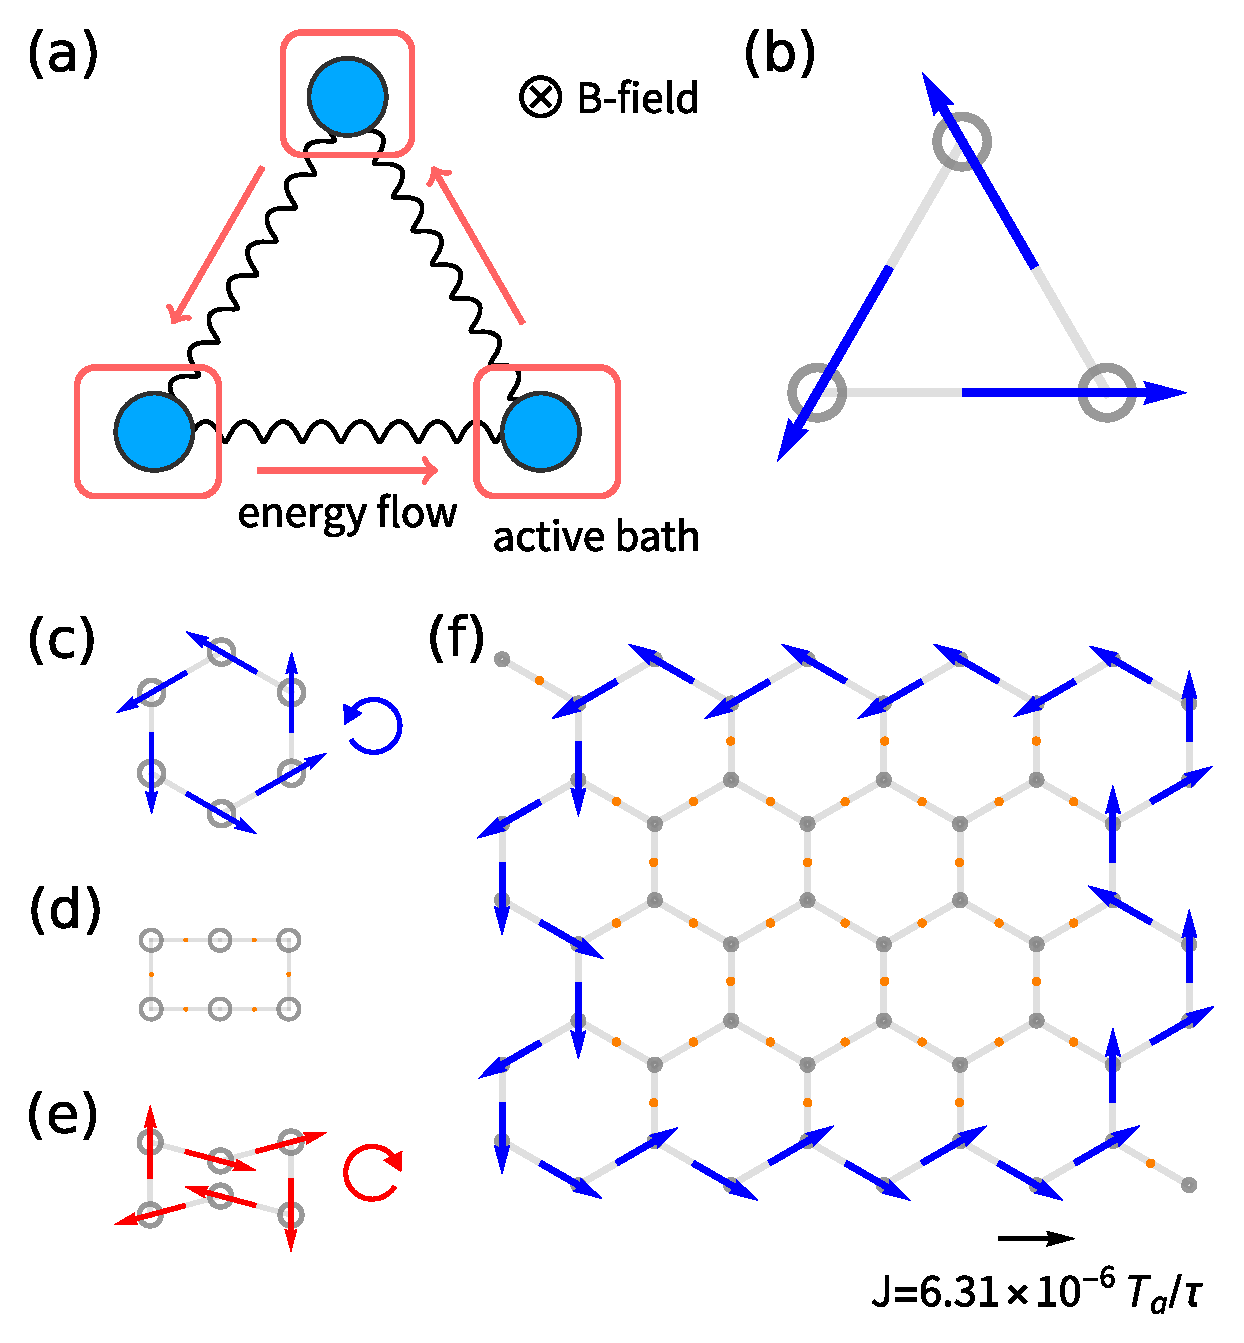
\includegraphics[width=0.45\textwidth]{1_model_and_result.pdf}
    \caption{The model and the heat flux in polygonal and more complex networks. All parameters are set to $1$.
    (a) Schematic of the model, a spring-mass network with Lorentz force and active bath on each mass.
    (b-f) Energy flux from numerical calculations. Gray circles and lines represent the network geometry. Arrows represent the direction and magnitude of the heat flux. Fluxes are colored blue if it is counter-clockwise (CCW), red if clockwise (CW), and orange otherwise. For complex networks, fluxes smaller than $1/10$ of the scale bar are not shown for clarity.
    (b) Triangle network has CCW heat flux, $\expval{J}=1.61\times 10^{-3} T_a/\tau$.
    (c-e) In hexagon networks, the flux direction changes with the geometry. Flux magnitude in both (c),(e) is $6.26\times 10^{-6} T_a/\tau$.
    (f) The flux pattern in the honeycomb network shows localization on the boundary and CCW direction.
    }
    \label{fig:model_and_result}
\end{figure}

Our model chiral system is a spring-mass network with Lorentz-like force and active bath \cite{Fodor2016HowFar} on each site (\figurename~\ref{fig:model_and_result}a).
The equation of motion reads
\begin{equation} \label{eqn:GLE_single}
    m\dot{\bm{v}}_i = -k_g \bm{z}_i + \sum_j\bm{F}_{ji} + \bm{v}_i\times\bm{B} - \gamma\bm{v}_i + \bm{\eta}_i ,
\end{equation}
where $z_i \equiv \begin{pmatrix} x_i & y_i \end{pmatrix}^T$ is the displacement of particle $i$ from its mechanical equilibrium position.

The first three terms on the right-hand side describe a spring-mass network with Lorentz force.
The first term is the on-site restoring force.
The second term is the spring force from the bonded neighbors $j$'s,
$F_{ji} = k (e_{ij}^T z_i + e_{ji}^T z_j) (-e_{ij})$.
Here the force is linearized by assuming the natural length of springs are much larger than the scale of particles' displacement, and $e_{ij}$ is the unit vector from the equilibrium position of $i$ to that of $j$.
The third term $\bm{v}_i\times\bm{B}$ is the Lorentz-like force (the electric charge-like factor is absorbed in $\bm{B}$), and we set $\bm{B} = -B\mathbf{\hat{z}}$.
The construction of our model system is motivated by the recently constructed topological gyroscopic metamaterials \cite{Nash2015TopologicalMechanics}. Indeed, in the linearized regime, the equations of our model system are equivalent to the equations of motion of the gyroscopic metamaterials~\cite{Lee2018TopologicalDynamics}.

The last two terms describe the active bath, which consists of friction $-\gamma v_i$ and an Ornstein-Uhlenbeck (OU) colored noise $\eta_i$~\cite{Fodor2016HowFar}.
The colored noise has finite correlation time $\tau$ and strength $T_a$ ($T_a$ has the unit of energy)
\begin{equation} \label{eqn:noise_correlation}
    \expval{\eta_i(t)\eta_{j}^T(t')} = I\delta_{i,j}\frac{\gamma T_a}{\tau} e^{-\frac{|t-t'|}{\tau}} ,
\end{equation}
where $I$ is the identity matrix with appropriate dimensions.
The time evolution of the OU noise can be described according to the following equation~\cite{Hanggi1994ColoredNoise},
\begin{equation} \label{eqn:noise_eom}
    \tau \dot{\eta}_i = -\eta_i + \sqrt{2\gamma T_a}\xi_i ,
\end{equation}
where $\xi_i$ is the standard Gaussian white noise.
The friction $-\gamma v_i$ and OU noise $\eta_i$ break fluctuation-dissipation relation, thus driving the system out of equilibrium~\cite{Fodor2016HowFar}.
The active bath reduces to the familiar Langevin bath in the $\tau \rightarrow 0$ limit.


\section{Energy flux definition and results} \label{sec:flux}

The observable we mainly focus on is the time-averaged energy flux between particles at steady state. For a system with pairwise interactions and on-site potentials, the energy flux $\expval{J_{ij}}$ from particle $i$ to $j$ reads
\begin{equation} \label{eqn:flux_def}
    \expval{J_{ij}} = \expval{\frac{1}{2} (\mathbf{v}_j \cdot \mathbf{F}_{ij} - \mathbf{v}_i \cdot \mathbf{F}_{ji})}
    = \expval{\mathbf{v}_j \cdot \mathbf{F}_{ij}}.
\end{equation}
To arrive at this formula, first we define the energy of a particle as the sum of its kinetic energy, on-site potential energy, and one half of the bond energies \cite{Lepri2003ThermalConduction}. Then we write down the energy balance relations using ideas from stochastic energetics~\cite{Sekimoto1998LangevinEquation}. Finally we identify the energy exchanged due to particle-particle interactions as the energy flux $\expval{J_{ij}}$. A detailed derivation is provided in the supplemental material.
We note that the energy flux can simply be interpreted as the rate at which work is done on particle $j$ by particle $i$.
Since this microscopic work is due to particles' stochastic motions, rather than due to an external control, the energy flux can also be interpreted as a heat flux \cite{Sekimoto1998LangevinEquation,Lepri2003ThermalConduction}. The energy fluxes are identitically equal to zero for a system at equilibrium.

Starting from the linear equations \eqnname~\eqref{eqn:GLE_single}, \eqref{eqn:noise_eom}, the energy fluxes can be solved numerically using methods introduced in \cite{Gardiner2009ItoCalculus,Ceriotti2010ColoredNoiseThermostats} (Supplemental Material).
A collection of numerical results are shown in \figurename~\ref{fig:model_and_result}. We see nonzero energy rectification or energy fluxes can be generated in our chiral active system (\figurename~\ref{fig:model_and_result}b), and the flux direction or pattern changes with the network geometry (\figurename~\ref{fig:model_and_result}c-f).
Using a linear response theory, we now develop analytical expressions for the energy flux. These expressions reveal how a combination of chirality, nonequilibrium activity, and network geometry is responsible for generating energy fluxes.


\section{Linear response theory for energy flux} \label{sec:linear_response}
We begin by writing the equations of motion, \eqnname~\eqref{eqn:GLE_single}, in frequency space,
\begin{gather} \label{eqn:response}
    \tilde{z}(\omega) = G^+(\omega) \tilde{\eta}(\omega), \\
    G^{+}(\omega) \equiv [K + i\omega(\gamma I + BA) - m\omega^2I]^{-1}.
\end{gather}
We represented the displacement of all particles by a column vector $z=\sum_i \ket{i}\otimes z_i$, with $\ket{i}$ denoting the 2D subspace of $i$, $\tilde{z}(\omega)$ denotes the Fourier transform of $z$. $\tilde{\eta}(\omega)$ is the Fourier transform of the OU noise, $G^+$ is the response matrix, matrix $K$ encodes all on-site and spring forces $F$ according to $F=-Kz$, and $A$ is an antisymmetric matrix $A=\sum_i \ket{i}\bra{i}\otimes \mqty(0 & 1 \\ -1 & 0)$. This equation describes how the displacement $z$ responses to the noise $\tilde{\eta}$.

Following the procedure in \cite{Kundu2011LargeDeviations}, the flux defined in \eqnname~\eqref{eqn:flux_def} can be expressed using $G^+$ as a spectral integral (Supplemental Material)
\begin{align}
    \expval{J} &= \int_{-\infty}^\infty \dd{\omega} h(\omega) J^{FT}(\omega), \label{eqn:flux_integral} \\
    J^{FT}(\omega) &\equiv -\frac{T_a k}{2\pi} \Re \tr G^+(\omega)A^{as}, \\
    h(\omega) &= \frac{1}{1+\omega^2\tau^2},
\end{align}
where $A^{as}$ is an antisymmetric matrix
$A^{as} = -\ket{i}\bra{j} \otimes e_{ij}e_{ji}^T + \ket{j}\bra{i} \otimes e_{ji}e_{ij}^T$.
The response function $G^+(\omega)$ has no pole in the lower-half complex plane, but the colored noise introduces one pole at $\omega = -i/\tau$. Using the residue theorem we get a compact expression for the energy flux (Supplemental Material)
\begin{equation} \label{eqn:flux_residue}
    \frac{\expval{J}}{T_a/\tau} = -\frac{k}{2} \tr G^+(-\frac{i}{\tau})A^{as} .
\end{equation}
\eqnname~\eqref{eqn:flux_integral} and \eqref{eqn:flux_residue} will serve as our starting point to understand the energy flux. While they contain all the information required to compute energy fluxes, they have limited utility as design principles. Indeed, as written down, they require that the flux be recomputed de novo for each new network geometry and non-equilibrium bath activity. In the next sections, we show that it is possible to expand \eqnname~\eqref{eqn:flux_integral} and \eqref{eqn:flux_residue} in forms that reveals desgin principles for controlling energy fluxes.

Before moving on, we note that the energy fluxes satisfy Kirchoff's law, $\sum_i \expval{J_{ij}} = 0$, i.e. on average there is no energy exchange between particles and the active bath. This can be shown by calculating the average heat exchange between particle $i$ and the active bath $\expval{\eta_i^T v_i - \gamma v_i^T v_i}$, which results in zero.
This Kirchoff's law puts a strong constraint on possible flux patterns among particles, and some corollaries immediately follow, such as networks with no cycles cannot have nonzero flux, and fluxes of all bonds in a polygon network (as in \figurename~\ref{fig:model_and_result}b-e) are equal.


\section{Ingredients for energy rectification and their roles} \label{sec:fourier}

Compared with an ordinary thermal spring-mass network, which supports no energy fluxes in its equilibrium steady state, our model contains two extra components, the Lorentz force and the correlation in the noise.
We first show that these two components provide two necessary ingredients required to ensure energy rectification in our model.

We interpret the functions $J^{FT}(\omega), h(\omega)$ in \eqnname~\eqref{eqn:flux_integral} as follows.
The function $J^{FT}(\omega)$ is proportional to the the energy flux at Fourier frequency $\omega$ in an isolated damped variant of our network.
The function $h(\omega)$ is proportional to the the noise spectrum, $\expval{\tilde{\eta}(\omega)\tilde{\eta}^*(\omega)} = 2\gamma T_a h(\omega) / t$.

To generate a nonzero flux, or equivalently make the integral nonzero, we need two requirements.
Firstly, $J^{FT}(\omega)$ should not be zero everywhere.
If $B=0$, the response $G^+$ is symmetric or reciprocal, and since $A^{as}$ is antisymmetric, the trace $\tr G^+(\omega) A^{as}=0$ at all values of $\omega$. Nonzero $B$ breaks the reciprocity of $G^+$, thus can generate a nonzero $J^{FT}(\omega)$, or generate chiral Fourier modes.

Nonzero $J^{FT}(\omega)$ alone does not ensure a nonzero flux, we further need that $h(\omega)$ should not be constant.
If $h(\omega)$ is constant, it corresponds to a white noise, and the system would be in equilibrium according to the Bohr-van Leeuwen theorem \cite{Pradhan2010NonexistenceClassical}.
The $h(\omega)$ for the fluctuation dissipation violating OU noise, $h(\omega)=1/(1+\omega^2\tau^2)$, provides more weightage to fluxes at smaller values of $\omega$. The resulting average flux can hence potentially be nonzero. We note that other forms of colored noise could have also served the same purpose.

In summary, we see that $B$-field, and a colored noise are two necessary ingredients to generate flux in our model chiral systems.
The role of the $B$-field is to breaking the reciprocity of response and generate Fourier modes such that $J^{FT}(\omega)\neq 0$. The role of the colored noise is to excite these modes in a weighted manner.

Apart from the these two ingredients, the geometry of the network also plays an important role.
Indeed in the small $\gamma$ regime, the existence of chiral modes with $J^{FT}(\omega)\neq 0$ can further be heuristically explained by exploiting the connection between the slightly damped isolated variants of our system and the undamped isolated gyroscopic metamaterials~\cite{Nash2015TopologicalMechanics,Mitchell2018AmorphousTopological}.
Specifically, the slightly damped variant would resonate near the eigen-frequencies of the undamped metamaterials, and exhibit Fourier modes that are close to the eigenmodes of the undamped system (\figurename~\ref{fig:Fourier_modes}a,b). Consequently, we infer that $J^FT(\omega)\neq 0$ as long as the corresponding eigenmodes in the undamped variant are chiral. As discussed in  \cite{Nash2015TopologicalMechanics}, the geometry of the network plays a crucial role in generating the chiral eigenmodes.
At larger $\gamma$'s, the Fourier modes of our damped isolated variant are no longer close to the chiral eigenmodes of gyroscopic metamaterials (\figurename~\ref{fig:Fourier_modes}a,c), but a connection between eigenmodes and energy fluxes can still be built (Supplemental Material).
In the next section, we further elaborate the role of geometry. Specifically, the central results of the next section provide compact expressions that elucidate the role played by geometry. These expressions account for the contribution to the flux from all the Fourier modes.

\begin{figure}[ht]
	\centering
	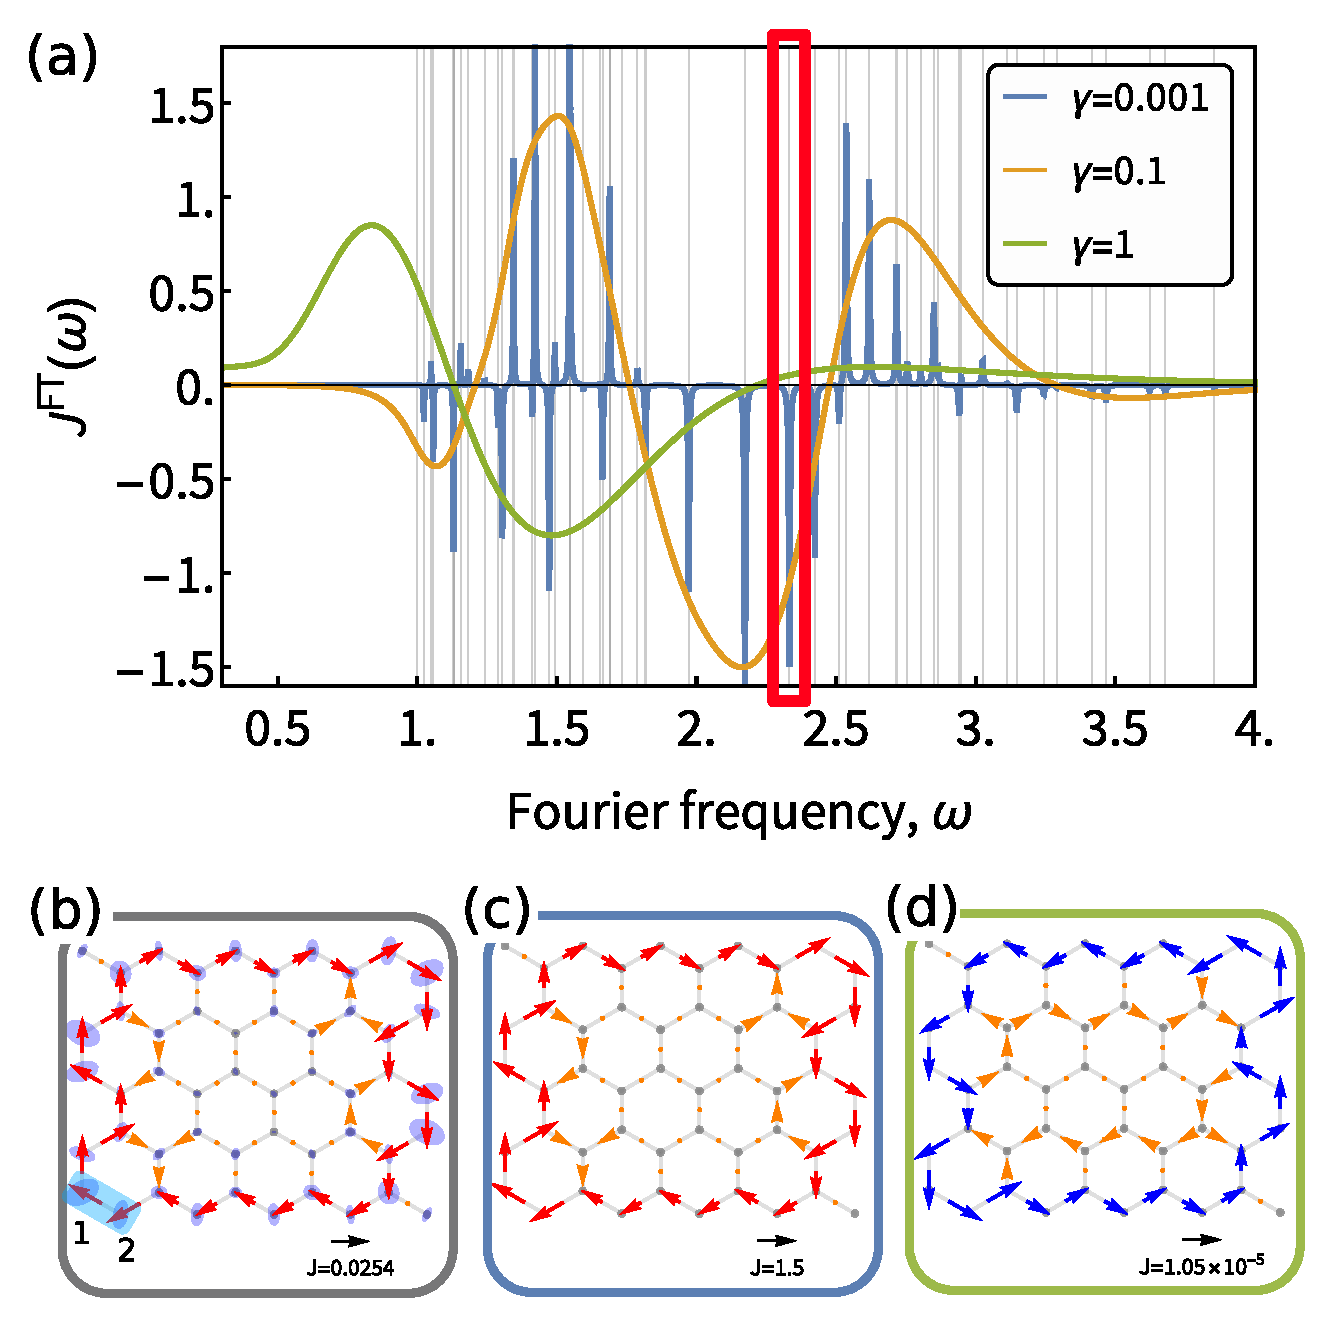
\includegraphics[width=0.45\textwidth]{2_Fourier_modes.pdf}
    \caption{Comparison between a boundary-localized eigenmode of the undamped isolated network and the Fourier modes of the damped network at the same frequency. First order dynamics (by setting $m=0$) are used. All other parameters are set to $1$.
    (a) Eigenmode of undamped gyroscopic system. For the frequency chosen, the eigenmode is localized on the boundary. Blue disks represent the orbit of particles.
    (b) The Fourier mode of damped variant of our model at small $\gamma$ ($\gamma=0.001$) resembles the eigenmode.
    (c) The Fourier mode at larger $\gamma$ ($\gamma=1$) is no longer close to the eigenmode.
    }
    \label{fig:Fourier_modes}
\end{figure}


\section{Relationship between flux and network geometry} \label{sec:path}
\begin{figure}[ht]
	\centering
	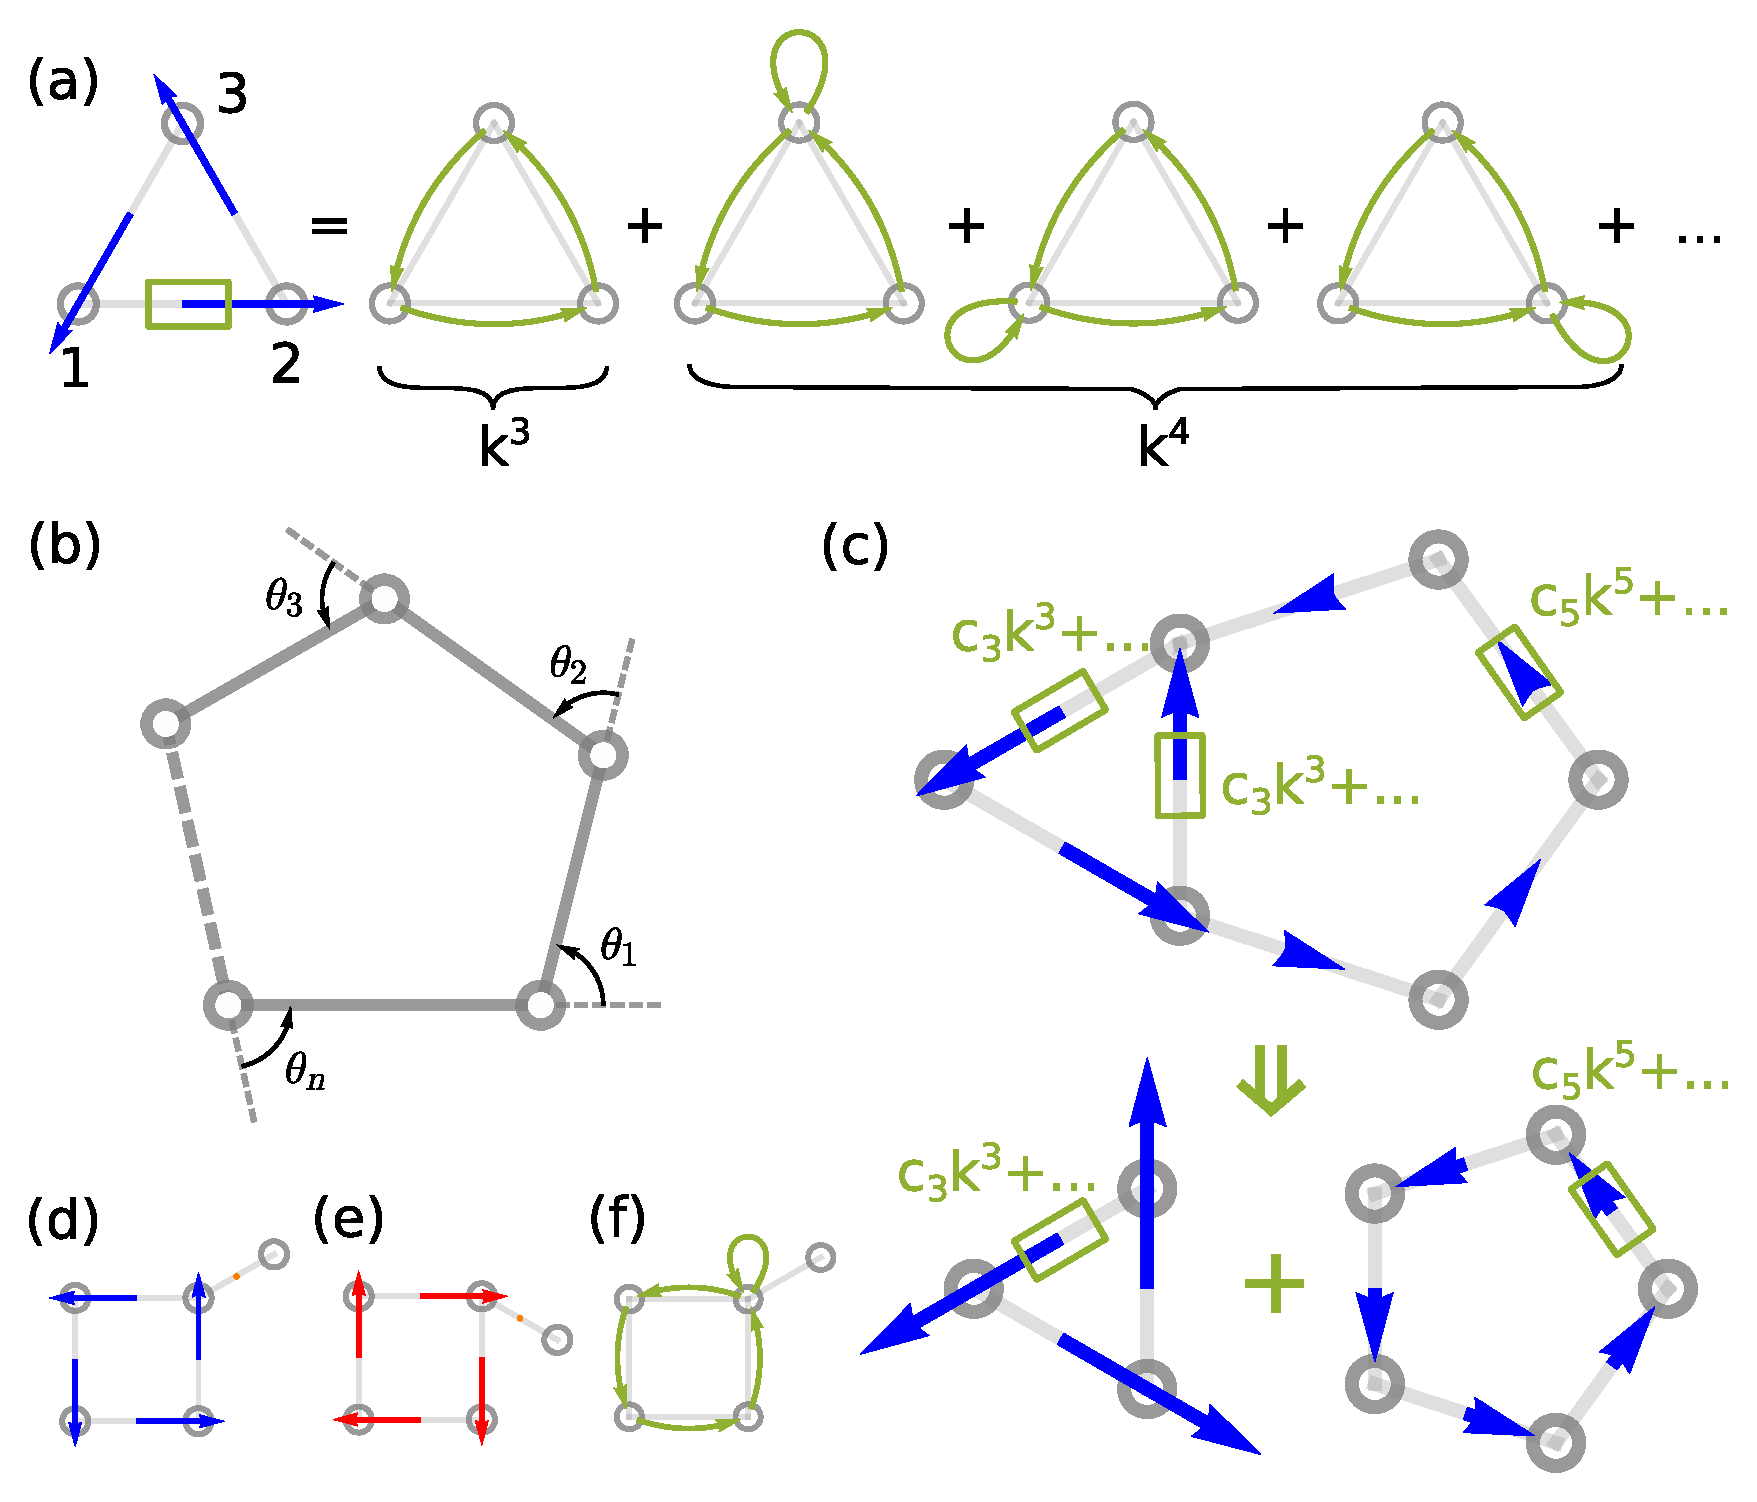
\includegraphics[width=0.45\textwidth]{4_path_sum.pdf}
    \caption{Illustrations of the path summation method.
    (a) Flux from $1$ to $2$ can be calculated by summing over paths. Each path is a diagrammatic representation of one term in the small-$k$ expansion, and is depicted using green arrows. The magnitude of path with length $n$ is on the order of $k^n$.
    (b) Schematic of a polygon path and its outer angles $\theta_1,\theta_2,\dots,\theta_n$. The flux of this path is simply \eqnname~\eqref{eqn:flux_path_polygon}.
    (c) For flux in complex networks, the leading order term is determined by the shortest cycles. Flux in the triangle part has order $k^3$, and the pre-factor $c_3$ is the same as that in a standalone triangle network. Likewise for the pentagon part. So the flux in a complex network can be viewed as a result of ``stitching" flux in its cyclic components together.
    }
    \label{fig:path_sum}
\end{figure}

In this section we develop a diagrammatic technique to compute the energy flux across a link in a chiral active network. This diagrammatic technique provides a simple intuitive method to compute energy fluxes and reveals a relationship between flux and network geometry. The diagrammatic technique is constructed by expanding the expressions for the energy flux \eqnname~\eqref{eqn:flux_residue} in small-$k$ regime and shows how the energy flux across a link can be expressed as a  sum over paths traversed along the network (\eqnname~\eqref{eqn:flux_path}). Our perturbation theory assigns a geometry dependent pre-factor for each path, thus elucidating the role played by network geometry in ensuring rectified energy fluxes (\eqnname~\eqref{eqn:flux_path_polygon}). Together, the central results of this section, \eqnname~\ref{eqn:flux_path}, \eqnname~\ref{eqn:flux_path_polygon} provide compact expressions that elucidate how geometry, $B$ field, and correlation time of the fluctuation dissipation relation violating OU noise, $\tau$, can combine to generate energy flows in networks with arbitrarily complex geometry and topologies.
%Although these quantitative conclusions are based on small-$k$ expansion, they also qualitatively agree with many numerical examples at larger $k$'s.


\subsection{Path summation and its rules}
Starting from the flux formula \eqnname~\eqref{eqn:flux_residue}, one can expand the flux to different orders in the spring constant $k$. Then for each order, one can further expand to different paths.
As a result, the total flux can be written as a sum over the flux of paths (\figurename~\ref{fig:path_sum}a), (Supplemental Material)
\begin{equation} \label{eqn:flux_path}
    \frac{\expval{J}}{T_a/\tau} = \sum_l J^\text{path}_l = \sum_l \frac{1}{2}(S_l - S_{-l}).
\end{equation}

The path rules are as follows.
For the flux from $i$ to $j$, valid paths are $l=i\rightarrow j\rightarrow l_3\rightarrow l_4\rightarrow \dots \rightarrow l_n\rightarrow i$, where $l_a$ and $l_b$ either has to be bonded or $l_a=l_b$. Paths that contain equal numbers of $i\rightarrow j$ and $j\rightarrow i$ do not contribute (e.g. path $i\rightarrow j\rightarrow i$), because either the path itself vanishes or it cancels with another path. As a result of this, paths appear as cycles.
The term $S_l$ is defined as $S_l \equiv (\frac{k}{k_0})^n \tr R_\alpha (-K_s)_{i l_n} \cdots R_\alpha (-K_s)_{l_3j} R_\alpha (-K_s)_{ji}$.
In this definition, $k_0\equiv \sqrt{(k_g+\gamma/\tau+m/\tau^2)^2 + (B/\tau)^2}$ sets the characteristic scale with dimension $k$. $R_\alpha$ is a CCW rotation by angle $\alpha$, defined as
\begin{equation} \label{eqn:path_alpha_def}
    \alpha = \arcsin{\frac{B/\tau}{k_0}}.
\end{equation}
The factor $\alpha$ condenses all the geometry independent parameters into one angle.
$(K_s)_{l_b l_a} \equiv \frac{1}{k}\bra{l_b}(K-k_gI)\ket{l_a}$ is a non-dimensionalized spring force on $l_b$ due to the displacement of $l_a$.
$-l$ means $l$ in the reversed order.
The interval of convergence depends on the geometry of the whole network as well as the parameter $\alpha$. The typical value of the upper bound of $\frac{k}{k0}$ ranges between $0.3$ and $0.6$.

The paths can be represented using diagrams, from which the flux $J^\text{path}_l$ can be calculated easily. For instance, the first diagram in \figurename~\ref{fig:path_sum}a represents the path $1\rightarrow 2\rightarrow 3\rightarrow 1$. To calculate $S_l$, one writes $(-K_s)_{l_bl_a}$ for each arrow $l_a\rightarrow l_b$, $R_\alpha$ for each node $l_a$, then multiply these matrices in the reversed order, and calculate the trace, e.g. $S_{1\rightarrow 2\rightarrow 3\rightarrow 1} = (\frac{k}{k_0})^3 \tr R_\alpha (-K_s)_{13} R_\alpha (-K_s)_{32} R_\alpha (-K_s)_{21}$. To get $S_{-l}$, one takes the result of $S_l$ and replace $\alpha$ by $-\alpha$. Finally, $J^\text{path}_l$ can be calculated from the difference between $S_l$ and $S_{-l}$.

\subsection{Contributions to energy flux from polygonal paths}
Path with length $n$ is on the order $(\frac{k}{k_0})^n$, so that in the small $k$ regime, the main contribution to the flux comes from the lowest-order paths.
The usual lowest-order paths are polygonal cycles with no loops (loops are self-connecting edges, $l_a\rightarrow l_a$). In this case, the formula for $J^\text{path}_l$ \eqnname~\eqref{eqn:flux_path} reduces to a simple form (Supplemental Material)
\begin{equation} \label{eqn:flux_path_polygon}
    J^\text{path}_\text{polygon} = \frac{1}{2} (\frac{k}{k_0})^n (\prod_i \cos(\theta_i - \alpha) - \prod_i \cos(\theta_i + \alpha)),
\end{equation}
where $\alpha$ is defined in \eqnname~\eqref{eqn:path_alpha_def}, $n$ is the number of nodes and $\theta_i$'s are outer angles (\figurename~\ref{fig:path_sum}b).
\eqnname~\ref{eqn:flux_path_polygon} illustrates how geometry of the network, as characterized by the angles $\theta_i$, together with the condensed parameter $\alpha$ that encodes the nonreciprocity due to the $B$ field and the violation of fluctuation dissipation due to the colored noise, combine to generate energy fluxes.

For polygon networks, \eqnname~\eqref{eqn:flux_path_polygon} gives a direct relationship between the lowest-order flux and the network geometry. As an example, flux in an arbitrary triangle is $J \propto k^3 \sin\theta_1\sin\theta_2\sin\theta_3 + \mathcal{O}(k^4)$, whose $k^3$ term is always positive or CCW.
For complex networks, \eqnname~\eqref{eqn:flux_path_polygon} implys that its lowest-order flux can be viewed as a result of combining the flux of its constituent polygons, as illustrated in \figurename~\ref{fig:path_sum}c. This is because the flux of a polygonal path \eqnname~\eqref{eqn:flux_path_polygon} is not affected by any side chains on the nodes, and $J^\text{path}_\text{polygon}$ for a polygon in a complex network is the same as $J^\text{path}_\text{polygon}$ for the polygon when standalone.

Starting from the  diagrammatic expansion, the presence of localized energy fluxes in some networks (\figurename~\ref{fig:model_and_result}) can be readily understood. Consider for instance the paths contributing to flux along an edge in a honeycomb-like network. Away from the boundary, the lower order path contributions to the energy flux cancel each other, and higher order path contributions become dominant. The size of the leading order path that contributes to the energy flux along a link increases as a function of the distance of the link from boundary. Such a scaling results in an exponential localization of the energy flux at the boundary of the network.

More generally, using these decompositions, it is easy to program energy flux patterns in networks of arbitrary complexity. Our diagrammatic expansion hence allows us to go beyond the need for de novo calculations suggested by our previous expressions.


\section{Coupling the energy flux to fluid pumping} \label{sec:swimmer}

\begin{figure}[ht]
	\centering
	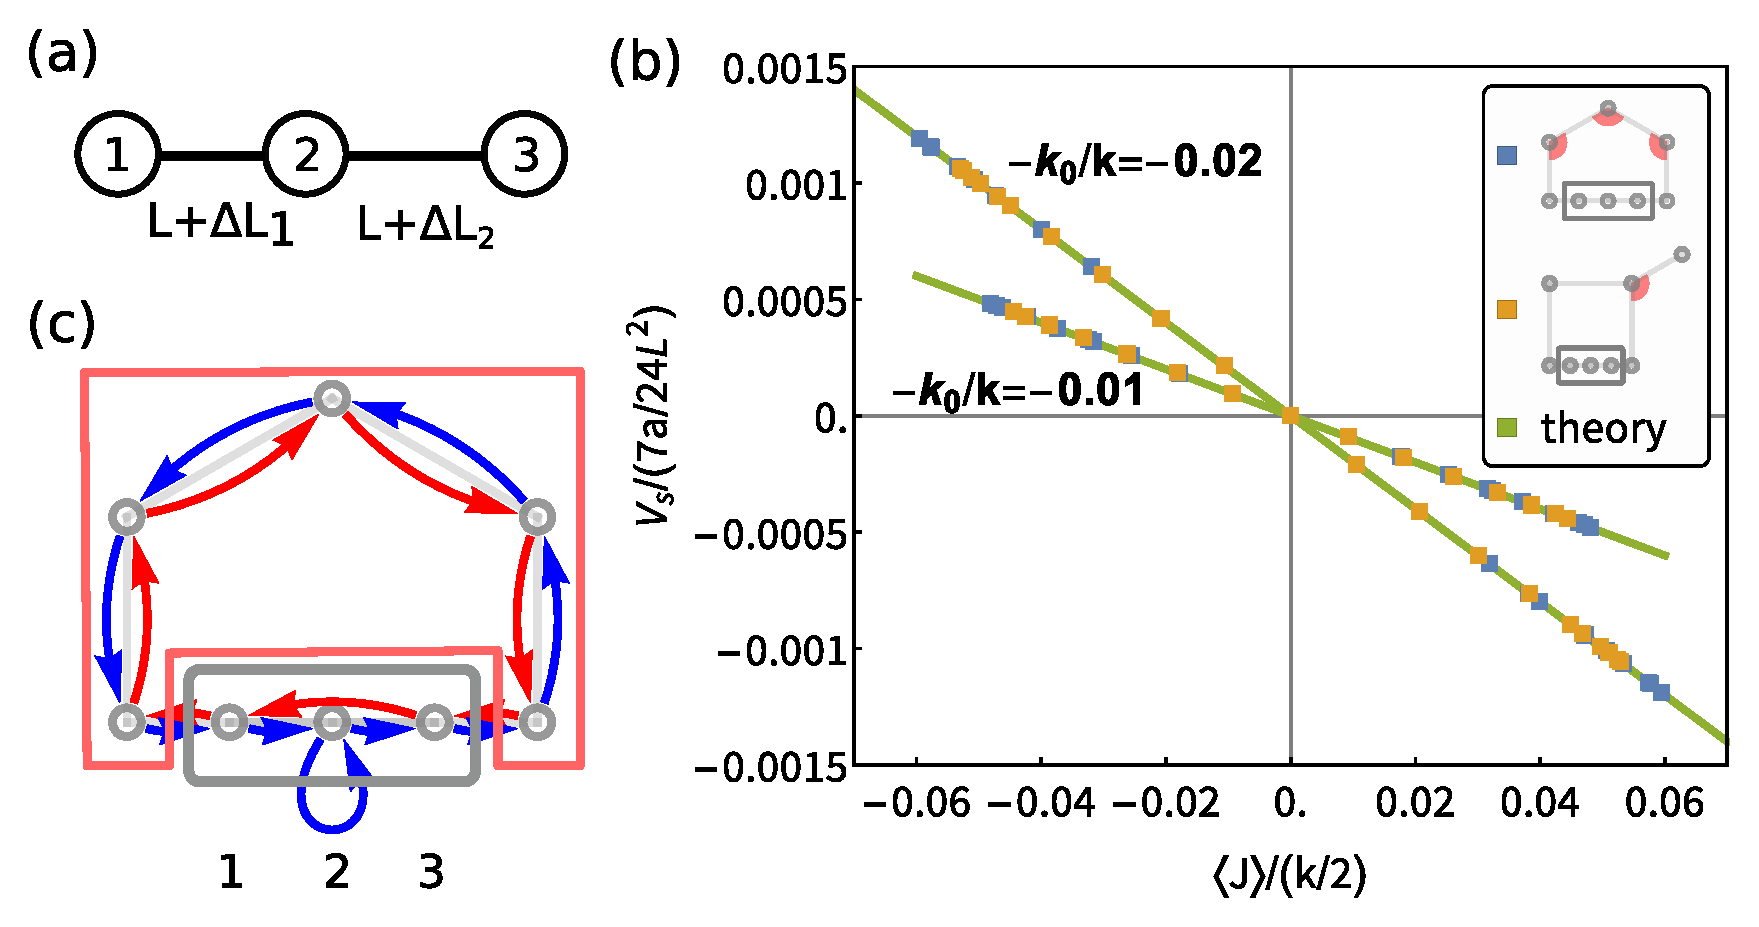
\includegraphics[width=0.45\textwidth]{7_swimmer.pdf}
    \caption{Active network dynamics as a swimming protocol.
    (a) Conventional heat conduction in a chain with temperature differences at two ends. The temperature difference drives a heat flow through a passive material (boxed in gray).
    (b) Similar to (a), the active gyroscopic network can also drive a heat flow through a passive segment. In the simulation setup, the separation between active particles (boxed in red) is large compared with the length-scale of their displacements, and their parameters are: $m,k_g,\gamma=0.1, k=10$, others are $1$. Passive particles (boxed in gray) are constrained to 1D, and their $\gamma,T_a,k_g$ are set to $0$.
    (c) Three-sphere swimmer model from \cite{Golestanian2008AnalyticResults}. In order to swim, the swimmer vary the lengths of its two legs according to some protocol.
    (d) Swimmer's speed $V_s$ is directly proportional to the energy flux $\expval{J}$ in the active network. The proportionality constant is $-k_0/k$, which is independent of the network geometry. The series of dots for each $-k_0/k$ are obtained by varying the labelled angles (by red disk sectors) in pentagon networks or square+tail networks.
    (e) One example of $J_{31}^s$ path (red) and $J_{12}^s$ path (blue). Ballistic particles are boxed in gray, and the active ones are boxed in red.
    }
    \label{fig:swimmer}
\end{figure}

The rectification of energy has been our main focus so far. In this section, we show that it possible to exploit the energy flux to rectify motions when our model systems are allowed to interact with a viscous fluid.
We begin by demonstrating that a {\it passive} segment \textendash this segment does not experience Lorentz force or active bath so that it is completely ordinary \textendash when coupled to our chiral active network, supports an energy flux.
Next we used the motion of this segment as input to construct a time dependent protocol to modulate the configuration of an equivalent segment that is disconnected from the network and placed in a viscous fluid. We find that doing so creates a low Reynolds number ($Re$) swimmer. Using the diagrammatic theory introduced in \secname~\ref{sec:path}, we show that the swimming speed is in fact proportional to the energy flux.
Using these results, we finally discuss the possibility that the energy conducting passive segment attached to our chiral active network, when immersed in a fluid, can act as a stalled swimmer and pump the fluid.

\subsection{Energy flux in a passive segment coupled to an active network}
We expect that our chiral active network can still generate energy fluxes when some nodes along the transmission pathway are made {\it passive} (i.e. uncoupled from the active bath and magnetic field).
Mimicking conventional paradigms to study heat conduction, which consider passive chain between two thermal baths with different temperatures (\figurename~\ref{fig:swimmer}a), we connect a passive harmonic chain to our chiral active network.
We indeed find that our chiral active network is able to generate a nonzero averaged energy flux through the passive material (\figurename~\ref{fig:swimmer}b, Supplemental Video and Supplemental Material).
From the Supplemental Video, the flux through the passive segment is in general stochastic. Although the direction of flux is from left to right on average, the instantaneous flux can also transport from right to left. During the period when $J$ is large, $J$ exhibits successive peaks, indicating a large energy flow from left to right. The spacing between the peaks matches the sound speed of the passive chain.


\subsection{Nonreciprocal motion as a swimming protocol}
The energy fluxes through the passive segment, especially the successive flux peaks observed in the above simulation, seem to suggest that stochastic wave like collective oscillations are responsible for the energy transfer. System with non-recriprocal wave-like fluctuations when placed in contact with a viscous fluid, can act as low $Re$ swimmers \cite{Taylor1951AnalysisSwimming,Purcell1977LifeLow,Golestanian2008AnalyticResults}. Thus, the nonreciprocal motion in the passive segment could potentially be exploited as a strategy to enable locomotion.

To pursue this idea, we consider a minimal passive elastic segment with three spheres arranged in a linear configuration~\cite{Golestanian2008AnalyticResults}. We imagine instances where the passive elastic segment is disconnected from the chiral active network and immersed in a low $Re$ fluid~\figurename~\ref{fig:swimmer}. When the lengths of the two springs connecting the spheres, $L+\Delta L_1(t), L+\Delta L_2(t)$ are varied according to some prescribed protocol, the time-averaged swimming speed is (\eqnname~(12) in \cite{Golestanian2008AnalyticResults})
\begin{equation} \label{eqn:swimmer_speed}
    V_s = \frac{7a}{24L^2} \expval{\Delta L_1 \Delta \Dot{L_2} - \Delta \Dot{L_1} \Delta{L_2}},
\end{equation}
where $a$ is the radius of the bead. Assumptions for this equation are $a/L \ll 1, \Delta L_i/L \ll 1$, and total external force on the swimmer is zero.

We now imagine recording the motions of the passive segment when it is connected to our chiral active network (\figurename~\ref{fig:swimmer}b) and not coupled to a viscous fluid. This recorded motion can be used a protocol for modulating the configuration of an equivalent {\it swimmer} passive segment that is placed in a viscous fluid.
We compute $V_s$ of the swimmer using \eqnname~\ref{eqn:swimmer_speed} and find that it is in fact proportional to the energy flux, $\expval{J}$, conducted through the passive segment when it is coupled to the chiral active network (\figurename~\ref{fig:swimmer}d). The nonreciprocal motions that is responsible for energy fluxes can also be used as a protocol to generate motion in a low $Re$ fluid.
The proportionality constant between the swim speed, $V_s$ and the energy flux, $\expval{J}$, can be calculated using a modified path analysis technique (Supplementary Material),
\begin{equation} \label{eqn:swimmer_propto}
    \frac{V_s}{7a/24L^2} = -\frac{k_0}{k} \frac{\expval{J}}{k/2},
\end{equation}
where $k_0 = k_g + m/\tau^2$ ($B,\gamma=0$ for the passive part).
This result \eqnname~\eqref{eqn:swimmer_propto} holds beyond small-$k$ regime because all orders of paths are considered (\figurename~\ref{fig:swimmer}e, and Supplementary Material).
\figurename~\ref{fig:swimmer}d and \eqnname~\eqref{eqn:swimmer_propto} together establish that one can dictate swimmer's speed from the energy flux of active networks.
Similar proportionality between $V_s$ and $J$ can be expected for other types of three-sphere swimmers, such as one where one sphere is much larger than the other two \cite{Golestanian2008ThreesphereLowReynoldsnumber}. This is because the swim speed $V_s$ is generically proportional to the area enclosed in the $\Delta L_i$ space \cite{Golestanian2009StochasticLow}. This area is also proportional to the energy flux $J$ (Supplemental Material).

\subsection{Coupling energy flux to fluid pumping}
Finally, we now consider the scenario where the passive segment is immersed in a fluid. Since the segment is tethered by $k_g$ and is connected to the tethered active part, it cannot swim indefinitely. However, a tethered, stalled swimmers can potentially pump the fluid \cite{Leoni2009BasicSwimmer}.
We would like to see whether our passive segment can, at least in theory, similarly act as a stalled swimmer and pump the fluid.
Specifically, we consider how the tethering force and the coupling to the fluid affects the dynamics of the segment.

In the presence of tethering forces, \eqnname~\eqref{eqn:swimmer_speed} for $V_s$ needs to be modified.
Ref. \cite{Golestanian2008AnalyticResults} discussed swimmer with a constant external force $F$, and its \eqnname~(39) says the modified swimming speed $V_s(F) = V_s + F/(6\pi\eta_f a)$, where $\eta_f$ is fluid's dynamic viscosity.
Since this result is obtained under linearized hydrodynamics, it also applies to our stochastic case granted that we replace $F$ by its averaged value $\expval{F}$.
This tells us that we can first consider the untethered case, then go to the tethered case using the above formula.

In the presence of an added fluid, we would like that the original dynamics is not altered too much, otherwise both the energy flux and the correlation in \eqnname~\eqref{eqn:swimmer_propto} would be distorted, and one cannot utilize the $V_s \propto -\expval{J}$ result.
So we need a regime where the fluid, in spite of having a low $Re$, is perturbative.
To make the fluid perturbative, we need the dissipation rate due to the viscous force to be much smaller than the energy flux through the segment. This can be expressed as $\eta_f a v^2 \ll J$, where $v$ is the characteristic velocity of the bead, $J$ is the energy flux in the absence of the fluid.
To satisfy low $Re$ condition, one needs $Re = \rho_f a v /\eta_f \ll 1$, where $\rho_f$ is fluid's density.
Writing these two conditions together, one gets $J \gg \eta_f a v^2 \gg \rho_f a^2 v^3$.
This condition ignored hydrodynamic interactions between the beads, because it is a higher-order perturbation with the order of $a/L$.
As a numerical example, this condition can be satisfied by setting $k=5\times 10^{-5} kg/s^2, k_g=1\times 10^{-6} kg/s^2$ for springs (value of optical trap), $a=10^{-6}m$ for all beads (size used in \cite{Leoni2009BasicSwimmer}), $T_a=10^{-18} J, \tau=1s$ for the active bath \cite{Wu2000ParticleDiffusion}, $\rho_f=10^3kg/m^3, \eta_f=10^{-3}kg/(m\cdot s)$ for liquid (water), and $B=10^{-5} kg/s$ for the $B$-field.
From numerical calculations, $v=3.8\times 10^{-6}m/s$, and the three scales are $J=5\times 10^{-19}J/s, \eta_f av^2=1.4\times 10^{-22}J/s, a^2v^3\rho_f=5.4\times 10^{-29}J/s$, which does exhibit scale separations.
If the separation between beads is $L=10^{-7}m$, calculated pumping speed is $1\times 10^{-8} m/s$.
This speed can be scaled up by increasing $T_a$.
The only suspicious parameter is $B$, which seems too strong in order to make $J$ sizable. To make practical use of this model, one should consider Lorentz force substitutes, such as gyroscopes.

These discussions together suggest that, if the passive part is immersed in a perturbative fluid, it can generate fluid flows.
Assuming the relaxation timescale of the active network is much faster than the timescale of swimming due to the small $V_s(F)$, one can expect the following process. Initially the passive part experiences $\expval{F}=0$, so it swims with speed $V_s$; as the part drifts, $\expval{F}$ increases and acts in the direction of $-V_s$; when $\expval{F} \approx -6\pi\eta_f a V_s$, the swimmer is stalled. The stalled swimmer pumps fluid in direction $-V_s \propto \expval{J}$.


\section{Conclusion} \label{sec:conclusion}

[Will be rewritten/revised after we converge on everything else]We have established that, our active gyroscopic network can rectify energy and control its rectification through network geometries.
At last, we discuss possibilities to extend this model and provide outlooks.

In our theoretical treatment, the parameters are assumed uniform for all particles and bonds, which is not necessary. We only need $\tau,T_a$ to be uniform, and other parameters $m, k_g, k, B, \gamma$. can be nonuniform.
If we add an additional white noise to the equation of motion \eqnname~\eqref{eqn:GLE_single}, the energy flux is not affected. As a comparison, in models that use OUP for directed particle transport, the additional white noise would usually suppress the rectification \cite{Bartussek1996PreciseNumerics}.

From Fourier mode analysis (\secname~\ref{sec:fourier}), the ingredients for nonzero energy fluxes are nonreciprocal response and weighted excitation.
The nonreciprocal response is introduced by Lorentz-like forces, and it makes theory tractable, since this force does not do work on the particles and is linear. The disadvantage is that its experimental realization is not easy.
Inspired by these two ingredients, one can try other ways to achieve rectifications.
One way is to replace the active particle with Lorentz force by active rotors. In this case the equation for energy flux \eqnname~\eqref{eqn:flux_integral} would contain extra terms, and since rotors themselves are active, the active bath is not needed.
Another possible way is to introduce nonlinearity, as nonlinearity can make nonreciprocal metamaterials  (cite nonreciprocal). This has been exploited to make thermal diodes. One could imagine a setup that replaces the springs with these nonreciprocal materials, and add active bath but not Lorentz force to the connecting sites.

% outlook
% active matter + network structure. cite Woodhouse's work, search for others.


\section*{Acknowledgements}
We thank many people.


\bibliography{reference}

\end{document}
